%#MAKEINDEX /usr/texbin/makeindex main
\documentclass[a4paper,10pt,twoside]{article}
%%\usepackage{program}
\usepackage{amsmath}
%\usepackage{ascmac}
%\usepackage[dvipdfmx]{graphicx}  % for EPS and PDF
\usepackage{url}
\usepackage{fancyvrb}
\usepackage{makeidx}
\usepackage{float}
\usepackage{listings}
\usepackage[colorlinks=true, linkcolor=blue]{hyperref}
%\usepackage{tgbonum}
\usepackage{utopia}
\usepackage[dvipsnames]{xcolor}
\usepackage{fancyhdr}

\usepackage{pdfpages}

\usepackage{vruler}  %% if vertical ruler (line number) is needed

\setcounter{secnumdepth}{4}
\setcounter{totalnumber}{6}
\usepackage{fancyhdr}
\usepackage{microtype}

\hoffset=0cm
\oddsidemargin=0cm
\evensidemargin=0cm
\textwidth=16cm
\topmargin=-1cm
\voffset=0cm
\textheight=24cm

\long\def\comment#1{}
\def\progenv{\baselineskip=10pt\tt\progspecial{`}\parindent=0.3cm}
\def\shellenv{\baselineskip=10pt\tt\progspecial{`}\parindent=0.3cm\nolineno}

\renewcommand{\topfraction}{.99}
\renewcommand{\bottomfraction}{.99}

\fancyhf{}
\fancyhead[LE,RO]{\bfseries\thepage}
\fancyhead[LE]{\textit{ESCAPE-2 - D2.3: High-Level Intermediate (HIR) Representation Specification}}
\fancyhead[RO]{\textit{ESCAPE-2 - D2.3: High-Level Intermediate (HIR) Representation Specification}}
\fancyfoot[LE,RO]{\thepage}
\renewcommand{\headrulewidth}{0.5pt}
\renewcommand{\footrulewidth}{0pt}
\fancyheadoffset[RE,LO]{\textwidth}
\pagestyle{fancy}


\def\openb{{\it [}}
\def\closeb{{\it ]}}

\def\DAG{$^\dagger$}
\def\DDAG{$^\ddagger$}
%
\newcommand{\concept}[1]{
\hypersetup{ 
	linkcolor={blue},
}
\hyperref[cp:#1]{#1}
}

\newcommand{\irrconcept}[1]{
\hypersetup{ 
    linkcolor={Emerald},
}
\hyperref[cp:#1]{#1}
}

\newcommand{\element}[1] {
\subsection{{\tt #1} element}
\label{cp:#1}
}

\newcommand{\model}[1] {
\subsection{{\tt #1} model}
\label{cp:#1}
}

\newcommand{\HIRContentsModel}[1]{
\subsubsection*{Contents model}
{\tt #1}}
%
\newenvironment{HIRChildElements}{
\subsubsection*{Child elements}
\begin{tabular}{|l|p{10cm}|c|}
\hline
 name & description & R/O/A \\ \hline\hline
}{\end{tabular}}
%
\newcommand{\HIRElementDef}[3]{
{\tt #1} & #2 & #3 \\ \hline }
%
\newenvironment{HIRAttributes}{
\subsubsection*{Attributes}
\begin{tabular}{|l|c|p{10cm}|c|}
\hline
name & type & description & R/O/A \\ \hline\hline
}{\end{tabular}}

\newcommand{\HIRAttrDef}[4]{
{\tt #1} & #2 & #3 & #4\\ \hline }

\newenvironment{HIRAttributesVal}{
	\subsubsection*{Attributes}
	\begin{tabular}{|l|c|p{8cm}|c | c|}
		\hline
		name & type & description & suppoted values & R/O \\ \hline\hline
	}{\end{tabular}}

\newenvironment{HIRIrrAttributesVal}{
	\subsubsection*{Irregular Grid Attributes}
	\begin{tabular}{|l|c|p{8cm}|c | c|}
		\hline
		name & type & description & suppoted values & R/O \\ \hline\hline
	}{\end{tabular}}


\newcommand{\HIRAttrValDef}[5]{
	{\tt #1} & #2 & #3 & #4 & #5\\ \hline }

% %
% % \newenvironment{HIRControlList}{
% % \subsubsection*{Control list}
% % The values for the name attribute and the child element of the {\tt namedValue} element are as follows:
% % \newline
% % \newline
% % \begin{tabular}{|l|p{10cm}|c|}
% % \hline
% %  name attribute & child element & R/O \\ \hline\hline
% % }{\end{tabular}}
%
% \newenvironment{HIRSpecifier}[3]{
% {\tt #1} & #2 & #3 \\ \hline }
%
% \newenvironment{HIRElementList}{
% \begin{tabular}{|l|p{10cm}|}
% \hline
%  element & format of the content \\ \hline\hline
% }{\end{tabular}}
%
% \newenvironment{HIRElementFormat}[2]{
% {\tt #1} & #2 \\ \hline }
%
% \newenvironment{HIROperations}{
% \begin{tabular}{|l|p{4cm}|l|}
% \hline
%  element & operator & operation \\ \hline\hline
% }{\end{tabular}}
%
% \newenvironment{HIROperation}[3]{
% {\tt #1} & #2 & #3 \\ \hline }
%
% \newenvironment{HIRDataTypeNames}{
% \begin{tabular}{|l|p{11cm}|}
% \hline
%  type name & description \\ \hline\hline
% }{\end{tabular}}
%
% \newenvironment{HIRDataTypeName}[2]{
% {\tt #1} & #2 \\ \hline }


\lstdefinestyle{default}{
	basicstyle=\footnotesize,
    escapeinside={\^}{\^},
    frame=leftline,
	stepnumber=1,
	numbersep=10pt,
	tabsize=4,
	showspaces=false,
	showstringspaces=false
}

%% End of Preemble

%\title{{\Huge HIR}\\
%Specification\\
%\vspace{2cm}
%Version 0.1\\ }

%\author{
%\Large ESCAPE\\
%}
%\date{\vspace{4cm}\Large \today}

\makeindex

\begin{document}

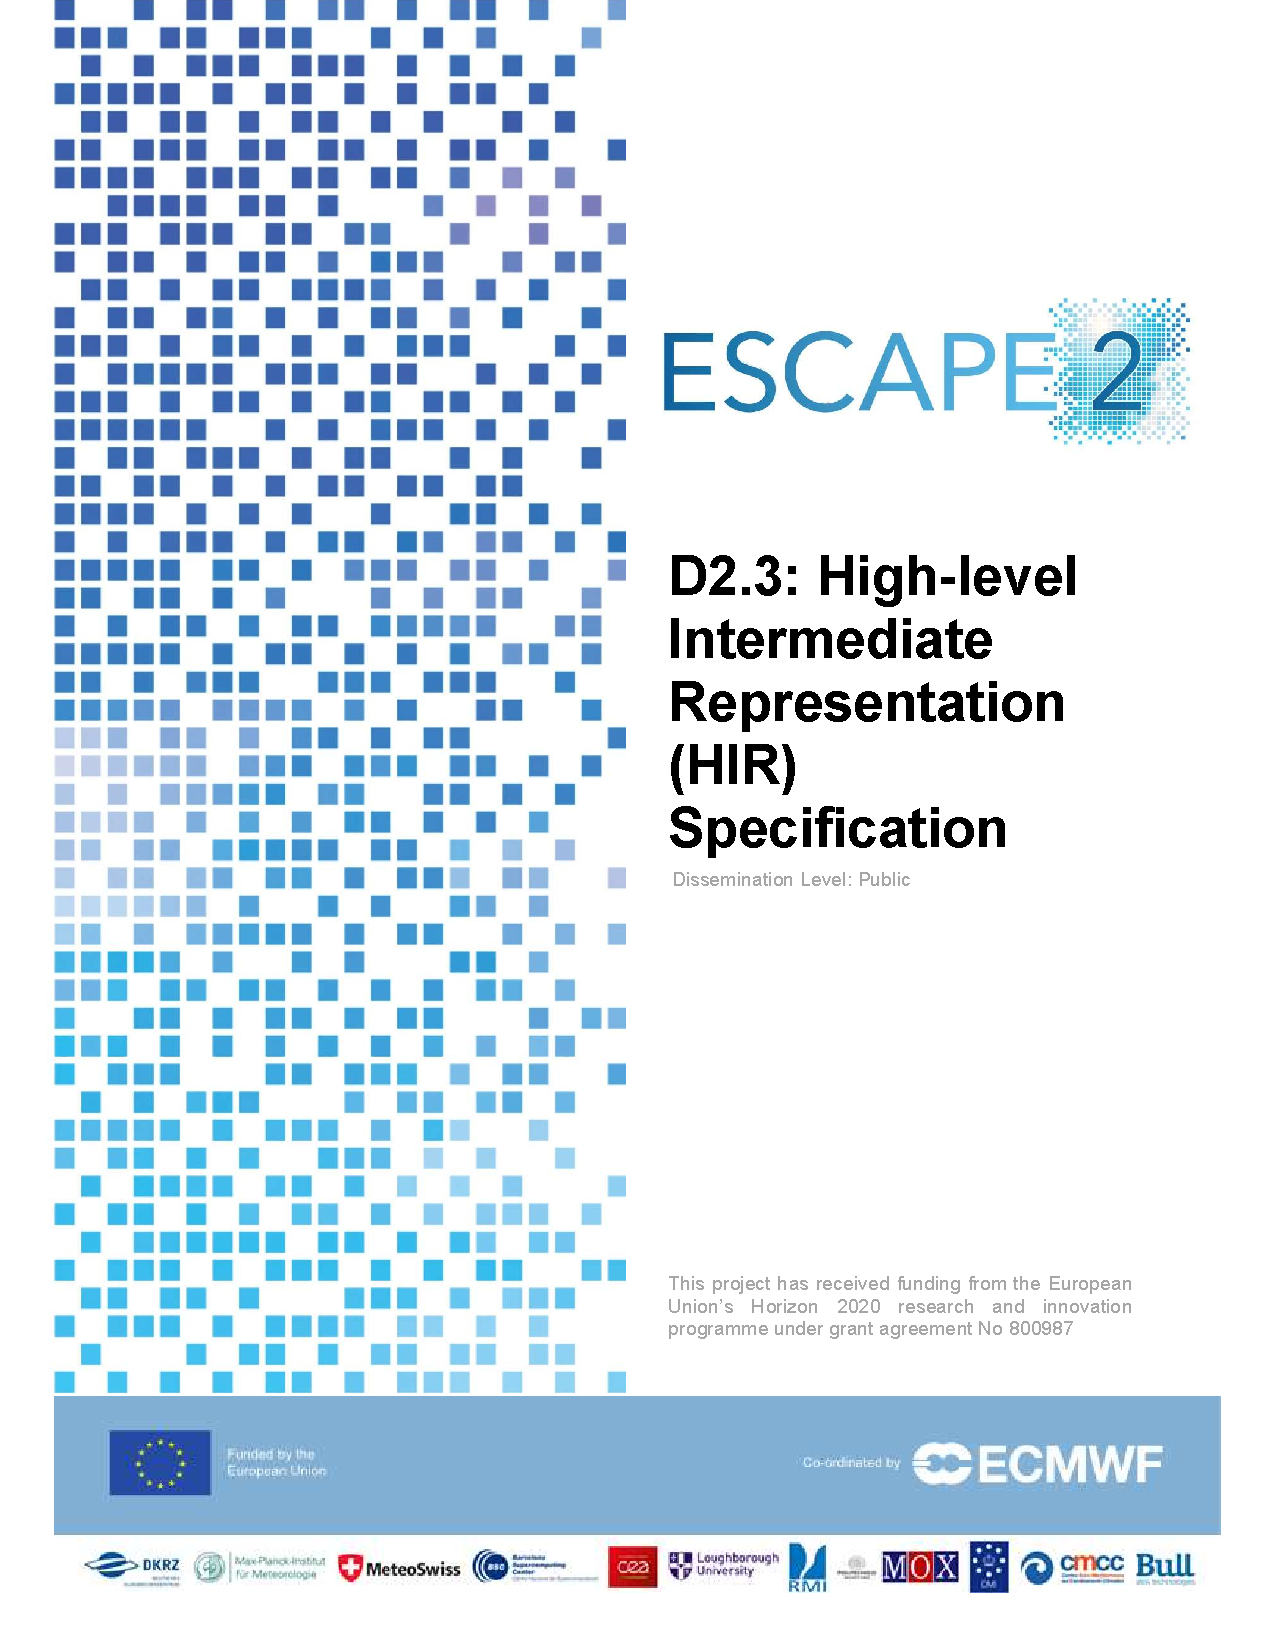
\includepdf[pages={1,2}]{./ESCAPE-2-D2-3_front_back.pdf}

\clearpage
%\input{history.tex}
\cleardoublepage


\tableofcontents
\listoffigures
\listoftables
%%%%\listoftables

%\input{ack.tex}

\newpage
\mbox{}\newpage

\section{Introduction}


This document provides a full specification of the HIR

\subsection{Conventions}

Some of the elements will allow to have different children type of nodes depending on the scope of the node.

There are two scopes: 
\begin{enumerate}
	\item control\_flow defines the scope of nodes where one or more of the parallel dimensions of the \concept{Domain} are not yet resolved within a \concept{Computation}
	\item domain\_computation is the scope of nodes where all the parallel dimensions of the \concept{Domain} are resolved within a \concept{Computation}
\end{enumerate}
\section{General HIR elements}

\element{Program}

Description of the element {\tt Program} element:

\subsubsection*{ContentsModel}{}

\begin{lstlisting}[style=default,frame=none]
(^\concept{GridDimension}^+,^\concept{Domain}^, ^\concept{FieldDecl}^+, ^\concept{VarDecl}^*, (^\concept{ScopedProgram}^|^\concept{ExternalKernel}^)+)
\end{lstlisting}

\begin{HIRChildElements}
\HIRElementDef{dimension}
{Definition of all the dimensions used within the program}{R}
\HIRElementDef{domain}
{specifies a domain that serves as hints to the compiler}{R}
\HIRElementDef{field}
{Definition of all the fields used by the program}{R}
\HIRElementDef{vararg}
{Definition of scalar variables arguments to the program}{O}
\HIRElementDef{ScopedProgram}
{a scoped program with computational patterns supported by the concepts of the HIR}{O}
\HIRElementDef{ExternalKernek}
{describes a kernel that contains computational patterns non supported by the concepts of the HIR}{O}
\end{HIRChildElements}

\begin{HIRAttributes}
\HIRAttrDef{HIRversion}{text}
{version of the HIR}{R}
\HIRAttrDef{DomainPolicy}{text}
{policy that defines the domain of the HIR}{R}
\HIRAttrDef{time}{text}
{Date and time of translation}{O}
\HIRAttrDef{language}{text}
{source language information}{O}
\HIRAttrDef{source}{text}
{source code information}{O}
\end{HIRAttributes}

\element{Domain}

The domain provides domain information of the application that is used as hints to the compiler toolchain.

\subsubsection*{ContentsModel}{}

\begin{lstlisting}[style=default,frame=none]
( DomainParallelDimensions, VerticalDimension, ParallelDimensions )
\end{lstlisting}

\begin{HIRChildElements}
	\HIRElementDef{DomainParallelDimensions}
	{list of of one or more \concept{GridDimension}+ representing the dimensions 
	 over the domain is parallelized}{R}
	\HIRElementDef{VerticalDimension}
	{contains the \concept{GridDimension} element representing the vertical 
	 dimension}{R}
	\HIRElementDef{ParallelDimensions}
	{list of \concept{GridDimension}* on which computations are embarrassingly 
	 parallel}{R}
\end{HIRChildElements}

\element{ScopedProgram}

The {\tt ScopedProgram} defines all the computations performed using concepts of the HIR

\subsubsection*{ContentsModel}{}

\begin{lstlisting}[style=default,frame=none]
(^\concept{BlockStmt}^)
\end{lstlisting}

\begin{HIRChildElements}
	\HIRElementDef{BlockStmt}
	{Block statement containing the sequence of statements that forms the computation of the program}{R}
\end{HIRChildElements}

\element{ExternalKernel}

The {\tt ExternalKernel} defines a call to an external kernel, for which computations description is not provided

\subsubsection*{ContentsModel}{}

\begin{lstlisting}[style=default,frame=none]
( Inputs, Outputs)
\end{lstlisting}

\begin{HIRChildElements}
	\HIRElementDef{Inputs}
	{list of \concept{FieldDecl} that represents the input fields}{R}
	\HIRElementDef{Outputs}
	{list of \concept{FieldDecl} that represents the output fields}{R}
\end{HIRChildElements}

\element{GridDimension}

The {\tt GridDimension} elements defines a dimension of a multidimensional space where fields are discretized and over which \concept{Computation}s iterate.

\HIRContentsModel{ () }
\begin{HIRAttributes}
	\HIRAttrDef{name}{text}
	{Name of the dimension}{R}
\end{HIRAttributes}

\element{DimensionLevel}

The {\tt DimensionLevel} it is used to specify a position (that is specified as a runtime argument to the \concept{Program}) in a given dimension

\subsubsection*{ContentsModel}{}

\begin{lstlisting}[style=default,frame=none]
(^\concept{VarAccess}^, ^\concept{Literal}^)
\end{lstlisting}

\begin{HIRChildElements}
	\HIRElementDef{VarAccess}
	{It uses a scalar variable of rank N where each element act as a marker, whose runtime values will store the positions within the extent of the dimension.}{R}
	\HIRElementDef{Literal}
	{It is a integer offset that shifts the position of the level with respect to the value of the VarAccess }{R}
\end{HIRChildElements}

\element{DimensionInterval}

The {\tt DimensionInterval} defines an interval on a dimension.

\subsubsection*{ContentsModel}{}

\begin{lstlisting}[style=default,frame=none]
(^\concept{DimensionLevel}^,^\concept{DimensionLevel}^)
\end{lstlisting}

\begin{HIRChildElements}
	\HIRElementDef{DimensionLevel}
	{position placeholder on a dimension that defines the begin and end of the interval}{R}
\end{HIRChildElements}

\element{Type}

The {\tt Type} defines the type of storage declarations
\HIRContentsModel{ () }

\begin{HIRAttributesVal}
	\HIRAttrValDef{name}{text}
	{any of the supported types}{(double,int,float)}{R}
\end{HIRAttributesVal}

\element{FieldDecl}
The {\tt FieldDecl} element defines a multidimensional field storage
\subsubsection*{ContentsModel}{}

\begin{lstlisting}[style=default,frame=none]
(^\concept{Type}^,^\concept{GridDimension}^+)
\end{lstlisting}

\begin{HIRChildElements}
	\HIRElementDef{GridDimension}
	{dimensions of the multidimensional space where the storage is defined}{R}
	\HIRElementDef{Type}
	{value type of the grid elements of the field}{R}
\end{HIRChildElements}

\begin{HIRAttributes}
	\HIRAttrDef{name}{text}
	{name of the field}{R}
\end{HIRAttributes}


\element{Offset}
The {\tt Offset} is the relative distance in a given \concept{GridDimension} to a neighbor grid point.

\subsubsection*{ContentsModel}{}

\begin{lstlisting}[style=default,frame=none]
(^\concept{GridDimension}^)
\end{lstlisting}

\begin{HIRChildElements}
	\HIRElementDef{GridDimension}
	{Identifies the dimension where the offset is computed}{R}
\end{HIRChildElements}

\begin{HIRAttributes}
	\HIRAttrDef{distance}{int}
	{relative distance in the given dimension of the offset}{R}
\end{HIRAttributes}

\element{Computation}
The {\tt Computation} defines an iteration loop over the specified \concept{GridDimension}s of the domain.

\subsubsection*{ContentsModel}{}

\begin{lstlisting}[style=default,frame=none]
((^\concept{GridDimension}^|^\concept{DimensionInterval}^)+,(^\concept{BlockStmt}^))
\end{lstlisting}

\begin{HIRChildElements}
	\HIRElementDef{GridDimension}
	{Specifies the dimensions where the computation is defined,
		convering the whole extent of the grid for that dimension}{O}
	\HIRElementDef{DimensionInterval}
	{Provides a specific range on a dimension to iterate over}{O}
	\HIRElementDef{BlockStmt}
	{Specifies the block with the list of statements that form the computation}{R}
\end{HIRChildElements}


\element{BoundaryCondition}
The {\tt BoundaryCondition} defines the strategy to apply a boundary condition to a field, if required.

\subsubsection*{ContentsModel}{}

\begin{lstlisting}[style=default,frame=none]
(^\concept{FieldDecl}^, ^\concept{BlockStmt}^)
\end{lstlisting}

\begin{HIRChildElements}
	\HIRElementDef{FieldDecl}
	{field subject of boundary condition}{R}
	\HIRElementDef{BlockStmt}
	{BlockStmt with statement that implement the boundary condition computation}{R}
\end{HIRChildElements}

\begin{HIRAttributes}
	\HIRAttrDef{distance}{int}
	{relative distance in the given dimension of the offset}{R}
\end{HIRAttributes}

\section{Statement elements}

\element{VarDecl}

The {\tt VarDecl} represents a N-dimensional scalar.
\HIRContentsModel{ (Type) }

\begin{HIRChildElements}
	\HIRElementDef{Type}
	{type of the variable n-dimensional variable}{R}
\end{HIRChildElements}

\begin{HIRAttributes}
	\HIRAttrDef{name}{text}
	{name of the variable}{R}
	\HIRAttrDef{ndims}{int}
	{number of dimensions of the variable}{R}
	\HIRAttrDef{isarg}{bool}
    {specifies if the variable is argument to the main program}{R}
	\HIRAttrDef{initialization}{string}
	{operation to initialize the variable}{0}
\end{HIRAttributes}

\element{IfStmt}
The {\tt IfStmt} is a statement element that defines an if condition.

\subsubsection*{ContentsModel}{}

\begin{lstlisting}[style=default,frame=none]
( Condition, Then, Else? )

where if (scope == domain_computation)
Condition = (^\concept{unaryOpModel}^|^\concept{binaryOpModel}^|^\concept{TernaryOp}^|^\concept{FieldAccess}^|^\concept{VarAccess}^|^\concept{Literal}^)
else
Condition = (^\concept{unaryOpModel}^|^\concept{binaryOpModel}^|^\concept{TernaryOp}^|^\concept{VarAccess}^|^\concept{Literal}^)
\end{lstlisting}

\begin{HIRChildElements}
	\HIRElementDef{Condition}
	{contains expression that defines the condition of the if block}{R}
	\HIRElementDef{Then}
	{contains a sequence of \concept{stmtModel} that compose the {\tt then} 
	 computation of the block}{R}
	\HIRElementDef{Else}
	{contains a sequence of \concept{stmtModel} that compose the {\tt Else} 
	 computation of the block}{O}
\end{HIRChildElements}

\element{BlockStmt}
The {\tt BlockStmt} is a statement element that defines an block (of statements).

\subsubsection*{ContentsModel}{}

\begin{lstlisting}[style=default,frame=none]
(^\concept{stmtModel}^+)
\end{lstlisting}

\begin{HIRChildElements}
	\HIRElementDef{stmtModel}
	{statement that composes the {\tt block} computation}{R}
\end{HIRChildElements}

\element{AssignmentStmt}

The {\tt AssignmentStmt} defines an assignment operation expression.

\subsubsection*{ContentsModel}{}

\begin{lstlisting}[style=default,frame=none]
(^\concept{lValueModel}^, ^\concept{exprModel}^ )
\end{lstlisting}


\begin{HIRChildElements}
	\HIRElementDef{lValueModel}
	{Specifies the left-hand side expression. 
	 Refer to \concept{lValueModel}.}{R}
	\HIRElementDef{exprModel}
	{Specifies the right-hand side expression. 
	 Refer to \concept{exprModel}.}{R}
\end{HIRChildElements}


\section{Expression elements}

\element{Literal}

The {\tt Literal} defines the specification of a literal.
\HIRContentsModel{ (Type) }

\begin{HIRChildElements}
	\HIRElementDef{Type}
	{type of the literal}{R}
\end{HIRChildElements}

\begin{HIRAttributes}
	\HIRAttrDef{value}{string}
	{value of the literal}{R}
\end{HIRAttributes}

\element{Binary operations}

The elements representing binary operators are described below and follows the
\concept{binaryOpModel}: 

\begin{tabular}{|l|p{4cm}|l|}
	\hline
	 element & operator & operation \\ \hline\hline
	 {\tt plusOp} & + & addition \\ \hline 
	 {\tt minusOp} & - & subtraction \\ \hline 
	 {\tt mulOp} & * & multiplication \\ \hline 
	 {\tt divOp} & / & division \\ \hline 
	 {\tt powerOp} & ** & power \\ \hline 
	 {\tt logicalAnd} & \&\& & logical AND \\ \hline 
	 {\tt logicalOr} & || & logical OR \\ \hline 
	 {\tt logicalEqual} & == & logical equality \\ \hline 
	 {\tt logicalNotEqual} & != & logical unequality \\ \hline 
	 {\tt logicalGt} & > & logical greater than \\ \hline 
	 {\tt logicalLt} & < & logical less than \\ \hline 
	 {\tt logicalGe} & >= & logical greater or equal than \\ \hline 
	 {\tt logicalLe} & <= & logical less or equal than \\ \hline 
\end{tabular}


\element{Unary operations}

The elements representing unary operators are described below and follows the
\concept{unaryOpModel}:

\begin{tabular}{|l|p{4cm}|l|}
	\hline
	 element & operator & operation \\ \hline\hline
	 {\tt unaryMinus} & - & sign inversion \\ \hline 
	 {\tt logNot} & ! & logical not \\ \hline 
	 {\tt incrementOp} & ++ & increment by one \\ \hline 
	 {\tt decrementOp} & -- & decrement by one \\ \hline 
\end{tabular}

\subsubsection*{ContentsModel}{}

\begin{lstlisting}[style=default,frame=none]
(exprModel)
\end{lstlisting}

\begin{HIRChildElements}
	\HIRElementDef{exprModel}
	{Specifies the operand expression. Refer to \concept{exprModel}}{R}
\end{HIRChildElements}

\element{TernaryOp}

The {\tt TernaryOp} defines an ternary operator expression.

\subsubsection*{ContentsModel}{}

\begin{lstlisting}[style=default,frame=none]
(exprModel, exprModel, exprModel)
\end{lstlisting}

\begin{HIRChildElements}
	\HIRElementDef{exprModel}
	{Specifies the condition of the operation as the first operand, the 
	 left-hand expression of the ternary operation as the second 
	 operand, the right-hand expression of the ternary operation as the third 
	 operand. Refer to \concept{exprModel}.}{R}
\end{HIRChildElements}

\begin{HIRAttributes}
	\HIRAttrDef{operator}{string}
	{operator being applied to the operands}{R}
\end{HIRAttributes}

\element{FctCall}
Built-in function call for mathematical functions.


\subsubsection*{ContentsModel}{}
\begin{lstlisting}[style=default,frame=none]
(exprModel+)
\end{lstlisting}


\begin{HIRChildElements}
	\HIRElementDef{exprModel}{Arguments of the function call.}{R}
\end{HIRChildElements}

\begin{HIRAttributes}
	\HIRAttrDef{name}{string}
	{function name: (abs, sqrt, sin, cos, tan, asin, acos, atan, exp, log)}{R}
\end{HIRAttributes}

\element{VarAccess}
The {\tt VarAccess} is a expression that defines an access to a \concept{VarDecl}

\subsubsection*{ContentsModel}{}

\begin{lstlisting}[style=default,frame=none]
(^\concept{Literal}^*)
\end{lstlisting}

\begin{HIRChildElements}
	\HIRElementDef{Literal}
	{access index of the var, when it is declared with more than 1 dimension}{O}
\end{HIRChildElements}

\begin{HIRAttributes}
	\HIRAttrDef{name}{string}
	{The var declaration that is being accessed in this expression}{R}
\end{HIRAttributes}

\element{FieldAccess}
The {\tt FieldAccess} is a expression that defines an (relative to each grid point) access to a field

\subsubsection*{ContentsModel}{}

\begin{lstlisting}[style=default,frame=none]
(^\concept{Offset}^+)
\end{lstlisting}

\begin{HIRChildElements} 
	\HIRElementDef{Offset}
	{An offset (relative to current grid position) used to de-reference the field access}{O}
\end{HIRChildElements}
\begin{HIRAttributes}
	\HIRAttrDef{name}{string}
	{The name of the field declaration that is being accessed in this expression}{R}
\end{HIRAttributes}

Notice that the {\tt FieldAccess} node is available only for 
Cartesian grids. 
An exception is for irregular grids, when accessing cell or vertex
location type neighbours of an edge, since the connectivity is always
regular in this case (with two neighbour elements per edge). 
Therefore the {\tt FieldAccess} is allowed for irregular grids
when the \concept{Offset} is specified on a \concept{GridDimension} with 
a non-edge \irrconcept{LocationType} and there the main 
dense dimension of the \concept{Computation} node is {\tt edges}.

\element{AbsoluteFieldAccess}
The {\tt AbsoluteFieldAccess} is a expression that defines a direct access to a grid point of a field, 
opposite to a \concept{FieldAccess} that
represents a relative access to a neighbour grid point.

\subsubsection*{ContentsModel}{}

\begin{lstlisting}[style=default,frame=none]
(^\concept{VarAccess}^|^\concept{FieldAccess}^)+
\end{lstlisting}

\begin{HIRChildElements} 
	\HIRElementDef{VarAccess}
	{Variable access that holds the index addressing the absolute field access}{A}
	\HIRElementDef{FieldAccess}
	{Field access that holds the index addressing the absolute field access}{A}
\end{HIRChildElements}
\begin{HIRAttributes}
	\HIRAttrDef{name}{string}
	{The name of the field declaration that is being accessed in this expression}{R}
\end{HIRAttributes}

\element{NeighbourReduce}
A reduction operation over near neighbours of certain  \irrconcept{LocationType}.

\subsubsection*{ContentsModel}{}

\begin{lstlisting}[style=default,frame=none]
(^\concept{GridDimension}^+,^\concept{Literal}^,^\concept{exprModel}^)
\end{lstlisting}

\begin{HIRChildElements} 
	\HIRElementDef{GridDimension}
	{the dimension of the neighbours where the reduction is applied}{R}
	\HIRElementDef{Literal}{the initial value of the reduction}{R}
	\HIRElementDef{exprModel}{the expression applied to the data of each neighbour grid point that is reduced using the binary operator}{R}
\end{HIRChildElements}
 
\begin{HIRAttributesVal}
	\HIRAttrValDef{op}{string}
	{A reduction arithmetic operator}{(add, mul, min, max)}{R}
\end{HIRAttributesVal}



\section{Common elements}
The definitions commonly used in an arbitrary element are shown in this Section.

\model{stmtModel}
The {\tt stmtModel} is commonly used for elements that refer statements.

\subsubsection*{ContentsModel}{}

\begin{lstlisting}[style=default,frame=none]
(^\concept{VarDecl}^|^\concept{IfStmt}^|^\concept{BlockStmt}^)
\end{lstlisting}


\model{exprModel}
The {\tt exprModel} is commonly used for elements that refer expression.

\subsubsection*{ContentsModel}{}

\begin{lstlisting}[style=default,frame=none]
where if (scope == domain_computation)    
    (^\concept{unaryOpModel}^|^\concept{binaryOpModel}^|^\concept{TernaryOp}^|^\concept{Literal}^|^\concept{FieldAccess}^|^\concept{VarAccess}^|^\concept{FctCall}^)
else
    (^\concept{unaryOpModel}^|^\concept{binaryOpModel}^|^\concept{TernaryOp}^|^\concept{VarAccess}^|^\concept{Literal}^|^\concept{FctCall}^)
\end{lstlisting}


\model{lValueModel}
The {\tt lValueModel} is commonly used for elements that refer left-hand side
expression.

\subsubsection*{ContentsModel}{}

\begin{lstlisting}[style=default,frame=none]
where if (scope == domain_computation)    
    (^\concept{VarDecl}^|^\concept{VarAccess}^|^\concept{FieldAccess}^)
else
    (^\concept{VarDecl}^|^\concept{VarAccess}^)
\end{lstlisting}


\model{binaryOpModel}
The {\tt binaryOpModel} is used for elements that refer to binary operations.


\subsubsection*{ContentsModel}{}

\begin{lstlisting}[style=default,frame=none]
(exprModel, exprModel)
\end{lstlisting}

\begin{HIRChildElements}
	\HIRElementDef{exprModel}
	{Specifies the left-hand expression as the first operand, the right-hand 
	 expression as the second operand. Refer to \concept{exprModel}.}{R}
\end{HIRChildElements}


\model{Common attributes}
Some elements may have the following attributes. 
\begin{HIRAttributes}
    \HIRAttrDef{lineno}{text}
    {Specifies the line number in the source program}{R}
    \HIRAttrDef{file}{text}
    {Specifies the source code file name}{R}
\end{HIRAttributes}


\section{Irregular Grid Elements}
This section described elements that are valid only for
the specification for models on irregular grid.

\element{LocationType}
Describes the location on a mesh element, 
used to identify positions of fields and operations on 
the grid.

\begin{HIRAttributesVal}
	\HIRAttrValDef{location}{text}
	{a location on a mesh}{(node,cell,edge)}{R}
\end{HIRAttributesVal}

\element{NeighbourReduce}
A reduction operation over near neighbours of certain  \irrconcept{LocationType}.

\subsubsection*{ContentsModel}{}

\begin{lstlisting}[style=default,frame=none]
(^\concept{GridDimension}^+,^\concept{Literal}^,^\concept{exprModel}^)
\end{lstlisting}

\begin{HIRChildElements} 
	\HIRElementDef{GridDimension}
	{the dimension of the neighbours where the reduction is applied}{R}
	\HIRElementDef{Literal}{the initial value of the reduction}{R}
	\HIRElementDef{exprModel}{the expression applied to the data of each neighbour grid point that is reduced using the binary operator}{R}
\end{HIRChildElements}

\begin{HIRAttributesVal}
	\HIRAttrValDef{op}{string}
	{A reduction arithmetic operator}{(add, mul, min, max)}{R}
\end{HIRAttributesVal}

\section{Example}

\begin{lstlisting}[style=default]
Program {
  dimension : [ncol, nlay, ngpt]
  domain : Domain {
    parallel_domain_dim : ncol
    vertical_dim : nlay
    parallel_dim : ngpt
  },
  field : FieldDecl {
    name : mu0, Dimension : [ncol]
  }
  field : FieldDecl {
    name : tau, Dimension : [ncol, nlay, ngpt]
  }
  field : FieldDecl {
    name : w0, Dimension : [ncol,nlay, ngpt]
  }
  field : FieldDecl {
    name : g, Dimension : [ncol,nlay, ngpt]
  }
  field : FieldDecl {
    name : Rdif, Dimension : [ncol,nlay]
  }
  field : FieldDecl {
    name : Tdif, Dimension : [ncol,nlay]
  }
  field : FieldDecl {
    name : Rdir, Dimension : [ncol,nlay]
  }
  field : FieldDecl {
    name : Tdir, Dimension : [ncol,nlay]
  }
  field : FieldDecl {
    name : Tnoscat, Dimension : [ncol,nlay]
  }
  vararg : VarDecl {
    type : int
    name : ncolbounds
    isarg : true
  }
  vararg : VarDecl {
    type : int
    name : nlaybounds
    isarg : true
  }  
  scope : ScopedProgram {
    // two_stream (Missing arg list, name of what is called, shouldn't inline stuff at this point)
    // adding_sw (same as up)
    // additional_step (same as up)
    // two_stream
    VarDecl {
      type : real
      name : mu0_inv
    }
    VarDecl {
      type : real
      name : mu0_inv
    }
    VarDecl {
      type : real
      name : gamma1
    }
    VarDecl {
      type : real
      name : gamma2
    }
    VarDecl {
      type : real
      name : gamma3
    }
    VarDecl {
      type : real
      name : gamma4
    }
    VarDecl {
      type : real
      name : alpha1
    }
    VarDecl {
      type : real
      name : alpha2
    }
    VarDecl {
      type : real
      name : k
    }
    VarDecl {
      type : real
      name : RT_term
    }
    VarDecl {
      type : real
      name : exp_minusktau
    }
    VarDecl {
      type : real
      name : exp_minus2ktau
    }
    VarDecl {
      type : real
      name : k_mu
    }
    VarDecl {
      type : real
      name : k_gamma3
    }
    VarDecl {
      type : real
      name : k_gamma4
    }

    BlockStmt {
      // Computation, this is the only stmt that we will express as a tree. 
      // From this on, pseudocode for the statements will be used
      ExprStmt { 
        AssignmentOp {
          lhs : VarAccess {
            name : mu0_inv
          }
          rhs : BinaryOp {
            lhs : Literal {
              type : real
              value : 1.0
            }
            rhs : VarAccess {
              name : mu0
            }
            operator : /
          }
        }
      }
      Computation {
        dimension : ngpt
        dimension : ncol
        dimension : DimensionInterval {
          dimension : nlay
          DimensionLevel {
            var_placeholder : VarAccess { 
              VarDecl { nlaybounds }
              Literal {0}
            }
            offset : 0
          }
          DimensionLevel {
            var_placeholder : VarAccess { 
              VarDecl { nlaybounds }
              Literal {1}
            }
            offset : 0
          }
        }
        BlockStmt {
          gamma1 = (8._wp - w0 * (5._wp + 3._wp * g)) * .25_wp
          gamma2 =  3._wp *(w0 * (1._wp - g) * .25_wp
          gamma3 = (2._wp - 3._wp * mu0 * g ) * .25_wp
          gamma4 =  1._wp - gamma3
          alpha1 = gamma1 * gamma4 + gamma2 * gamma3 
          alpha2 = gamma1 * gamma3 + gamma2 * gamma4 
          k = sqrt(max((gamma1 - gamma2) * (gamma1 + gamma2), 1.e-12_wp))
          exp_minusktau = exp(-tau * k)
          exp_minus2ktau = exp_minusktau * exp_minusktau
          RT_term = 1._wp / (k * (1._wp + exp_minus2ktau)  + gamma1 * (1._wp - exp_minus2ktau) )
          Rdif = RT_term * gamma2 * (1._wp - exp_minus2ktau)
          Tdif = RT_term * 2._wp * k * exp_minusktau
          Tnoscat = exp(-tau * mu0_inv)
          k_mu     = k * mu0
          k_gamma3 = k * gamma3
          k_gamma4 = k * gamma4
          RT_term =  w0 * RT_term/merge(1._wp - k_mu*k_mu, epsilon(1._wp), abs(1._wp - k_mu*k_mu) >= epsilon(1._wp))
          Rdir = RT_term  * ((1._wp - k_mu) * (alpha2 + k_gamma3) -  (1._wp + k_mu) * (alpha2 - k_gamma3) * exp_minus2ktau - 2.0_wp * (k_gamma3 - alpha2 * k_mu)  * exp_minusktau  * Tnoscat)
          Tdir = Tnoscat - RT_term * ((1._wp + k_mu) * (alpha1 + k_gamma4) * Tnoscat - (1._wp - k_mu) * (alpha1 - k_gamma4) * exp_minus2ktau * Tnoscat - 2.0_wp * (k_gamma4 + alpha1 * k_mu)  * exp_minusktau)
          Tdir -= Tnoscat
        }   
      }
    }
  }
}
\end{lstlisting}


\section{Document History}

\begin{tabular}{|l|l|l|l|}
	\hline
	Version & Author(s) & Date & Changes \\ 
	&&& \\  \hline
	1.0 & Carlos Osuna (MSWISS) & 09/09/2019 & Compilation and edit of all contributions \\ \hline
\end{tabular}

\section{Internal Review History}

\begin{tabular}{|l|l|l|}
	\hline
	Internal Reviewers & Date & Comments \\ 
\hline
\end{tabular}

\section{Effort Contributions per Partner}
\begin{tabular}{|l|l|}
	\hline
	Partner& Efforts \\ 
	\hline
\end{tabular}

\includepdf[pages={4}]{./ESCAPE-2-D2-3_front_back.pdf}

\cleardoublepage

\end{document}
